\section{Atmospheric Radiation Measurement}
\subsection{Introduction to ARM program}
For 30 years and counting since its inception in 1990
\cite{Turner_AMS_2016}, ARM program has
been collecting observations across the globe to advance the robust
predictive understanding of Earth's climate and environmental systems
and to inform the development of sustainable solutions to the Nation's
energy and environmental challenges. Deployed across three atmospheric
observatories, three mobile facilities and aerial facilities, data are
continuously being collected from 480 scientific instruments and
sensors. With 1.7 Petabyte and growing archive of data, ARM makes
available to the scientific community, publicly and freely,
approximately 8218 data streams of which 1220 are actively growing in
near-real-time with data streaming from the instruments around the
world.

\begin{figure*}
 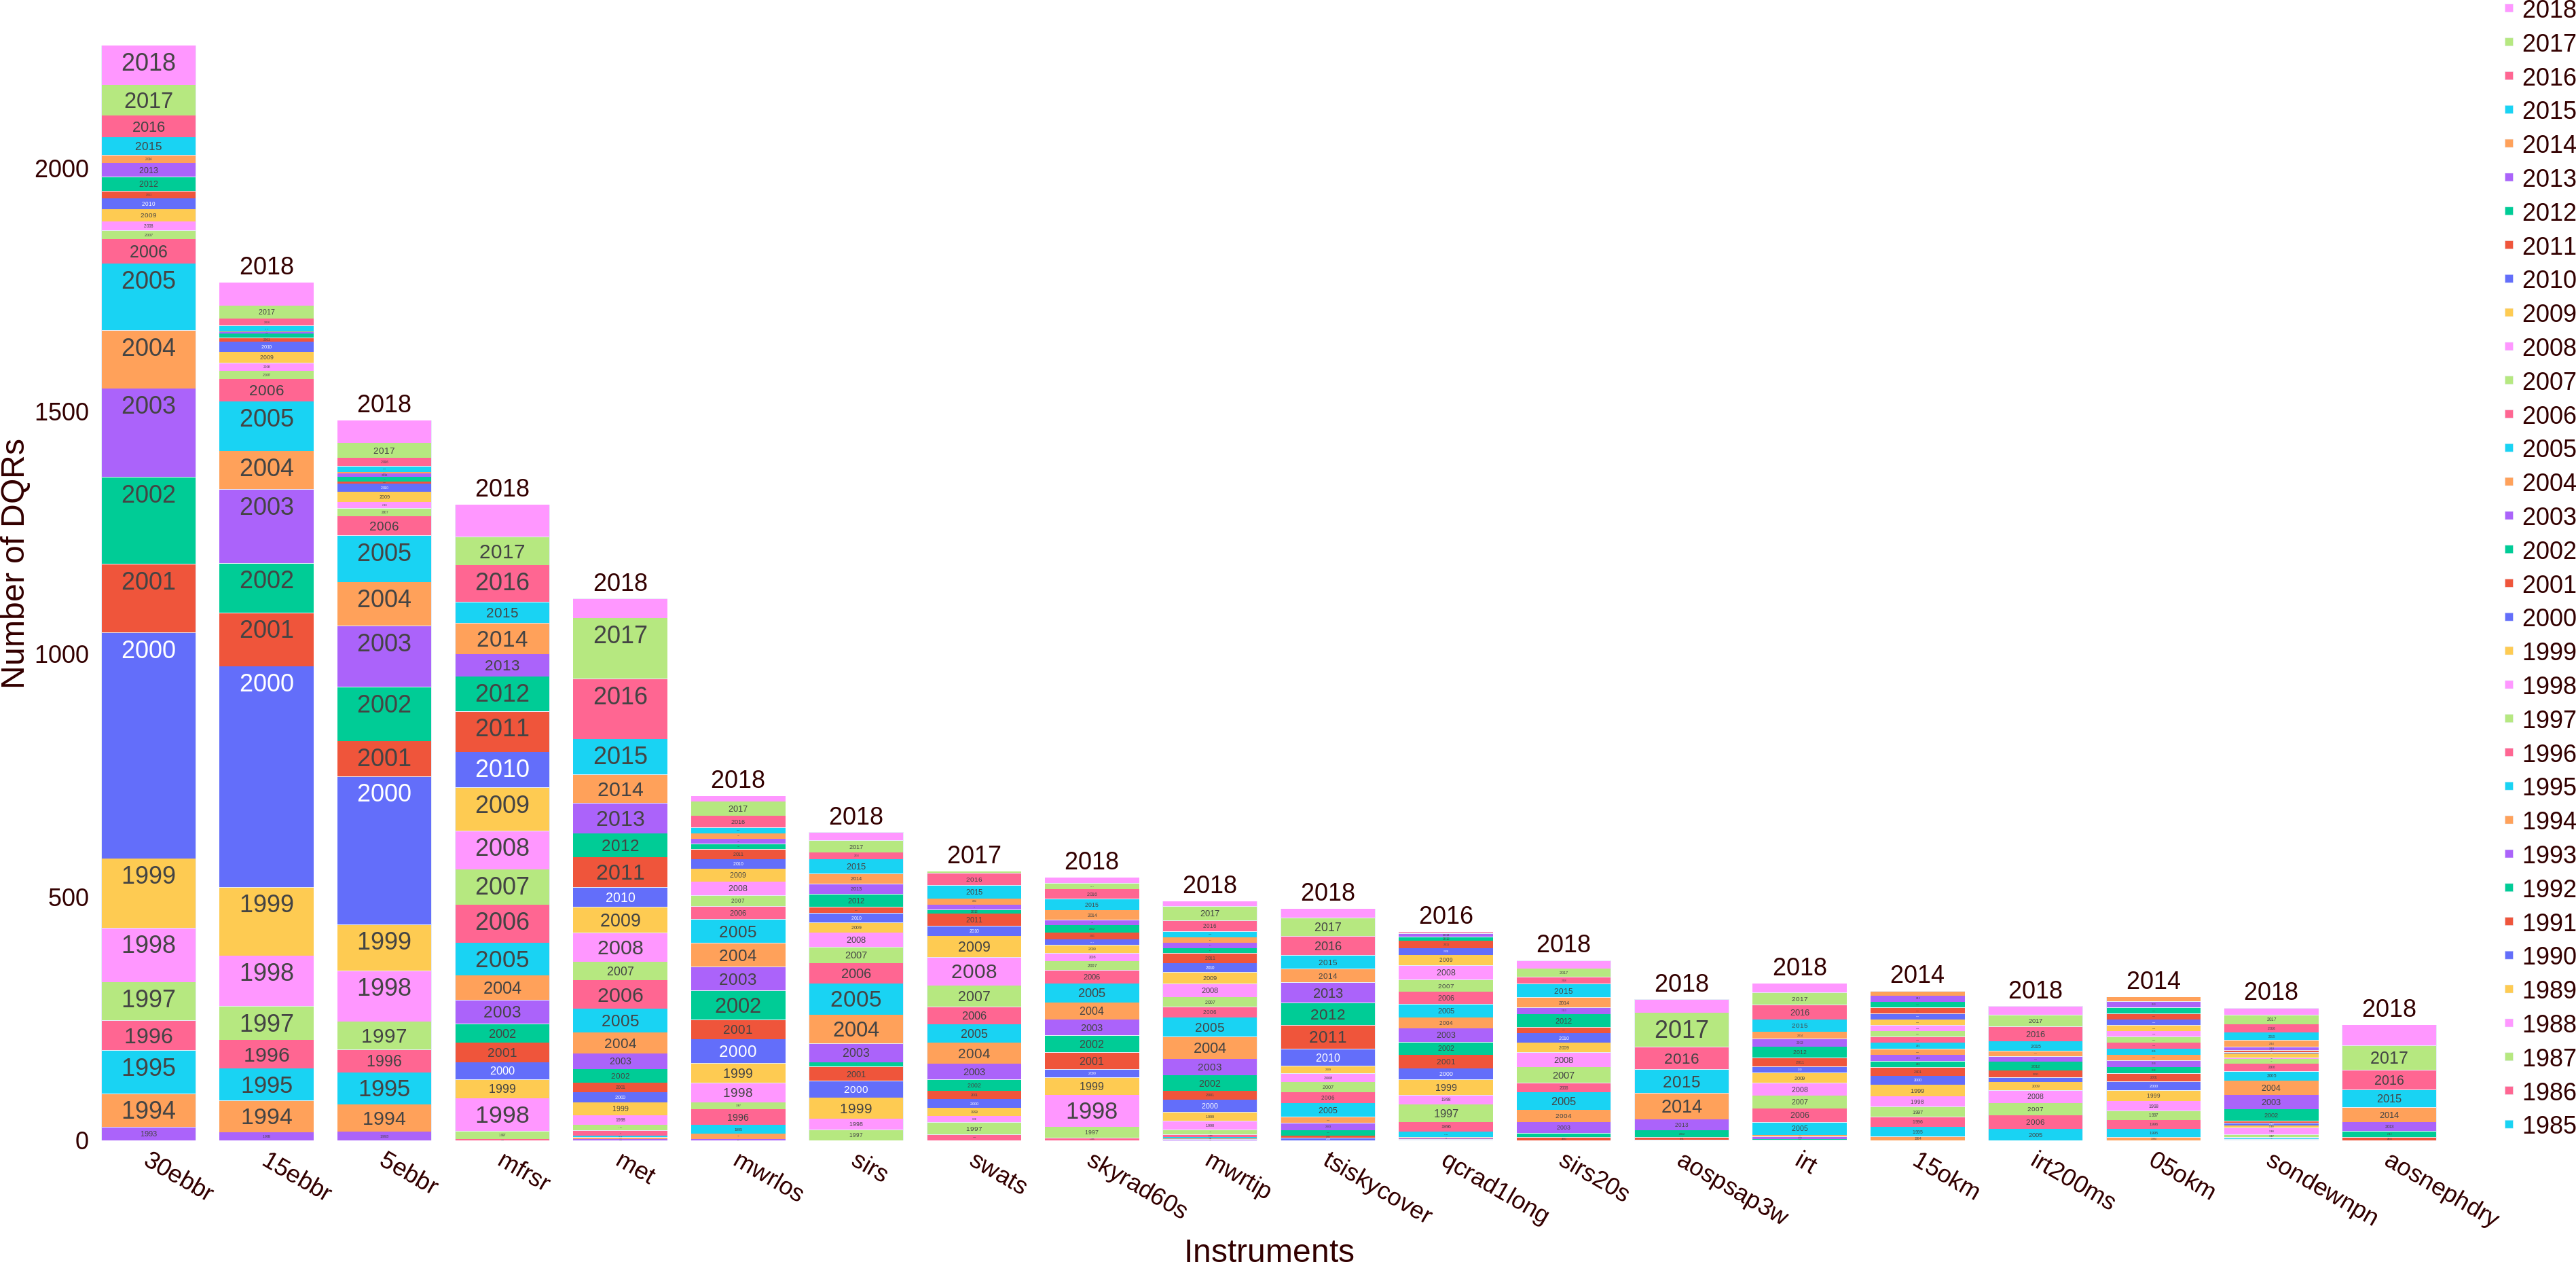
\includegraphics[width=\linewidth]{figures/dqr_by_instrument_20.png}
 \caption{DQRs for select 20 instruments over the period 1993-2019 show
 that some instruments are more prone to data quality issues than
 the others. Time series of DQRs show that data quality issues at many
 of the instruments are repetitive and recurring.}
 \label{fig:dqr_by_instrument}
\end{figure*}


\subsection{Assessment and Management of Data Quality}
These instruments for atmospheric observations, however, are prone to data quality issues due to
the challenging operating conditions in field
%(Figure~\ref{fig:dqr_by_instrument})
, sensor failures, need for
re-calibration etc. ARM Data Quality Office, established in year 2000,
coordinates detection and reporting of data quality for all data streams
\cite{Peppler_AMS_2016,peppler2005,peppler2008quality}.


Data Quality Reports (DQR) can be submitted by data quality analysts,
instrument mentors, facilities operations personnel or data users and
are saved within a consistent and searchable PostgreSQL database.
However, with large numbers of instruments and streaming data stream
maintained by the program, DQRs can be frequent and many. 
Figure~\ref{fig:dqr_by_instrument} shows the reported data quality
issues for 20 ARM instruments over time. Some instruments are more prone
to data quality issues than, often due to the nature of deployed
sensors, and its essential that the data be reprocessed to ensure the
availability of high quality continuous time series. Within ARM program,
reprocessing of data is conducted whenever a data quality issue that can
be corrected is identified. Reprocessing is also conducted if an
improved processing algorithm is available. However, the volume and
diversity of data poses a challenge.

Historically the complexity of data reprocessing to address the quality
issues, data size and volume has limited the improvements made to
correct for the data quality issue
(Figure~\ref{fig:dqr_instrument_per_year}). For example, 30 minute
resolution energy balance Bowen Ratio (30EBBR)
instruments that have been in operation since 1993 has largest number of
DQRs, most of which have not been addressed. Surface meteorology (MET)
observations, which are one of highly used datasets, had large number of
reported quality issues, only few of which has been corrected. In
contrast, radiation measurements (RAD) instruments had very few quality
issues, most of which were collected. 

\begin{figure}
 \centering
 \subfloat[30 minute Energy Balance Bowen Ratio (EBBR) instruments are
 one of the longest running core instruments within ARM and while it had
 a number of reported data quality issues every year, most of them have
 not been addressed.]{
  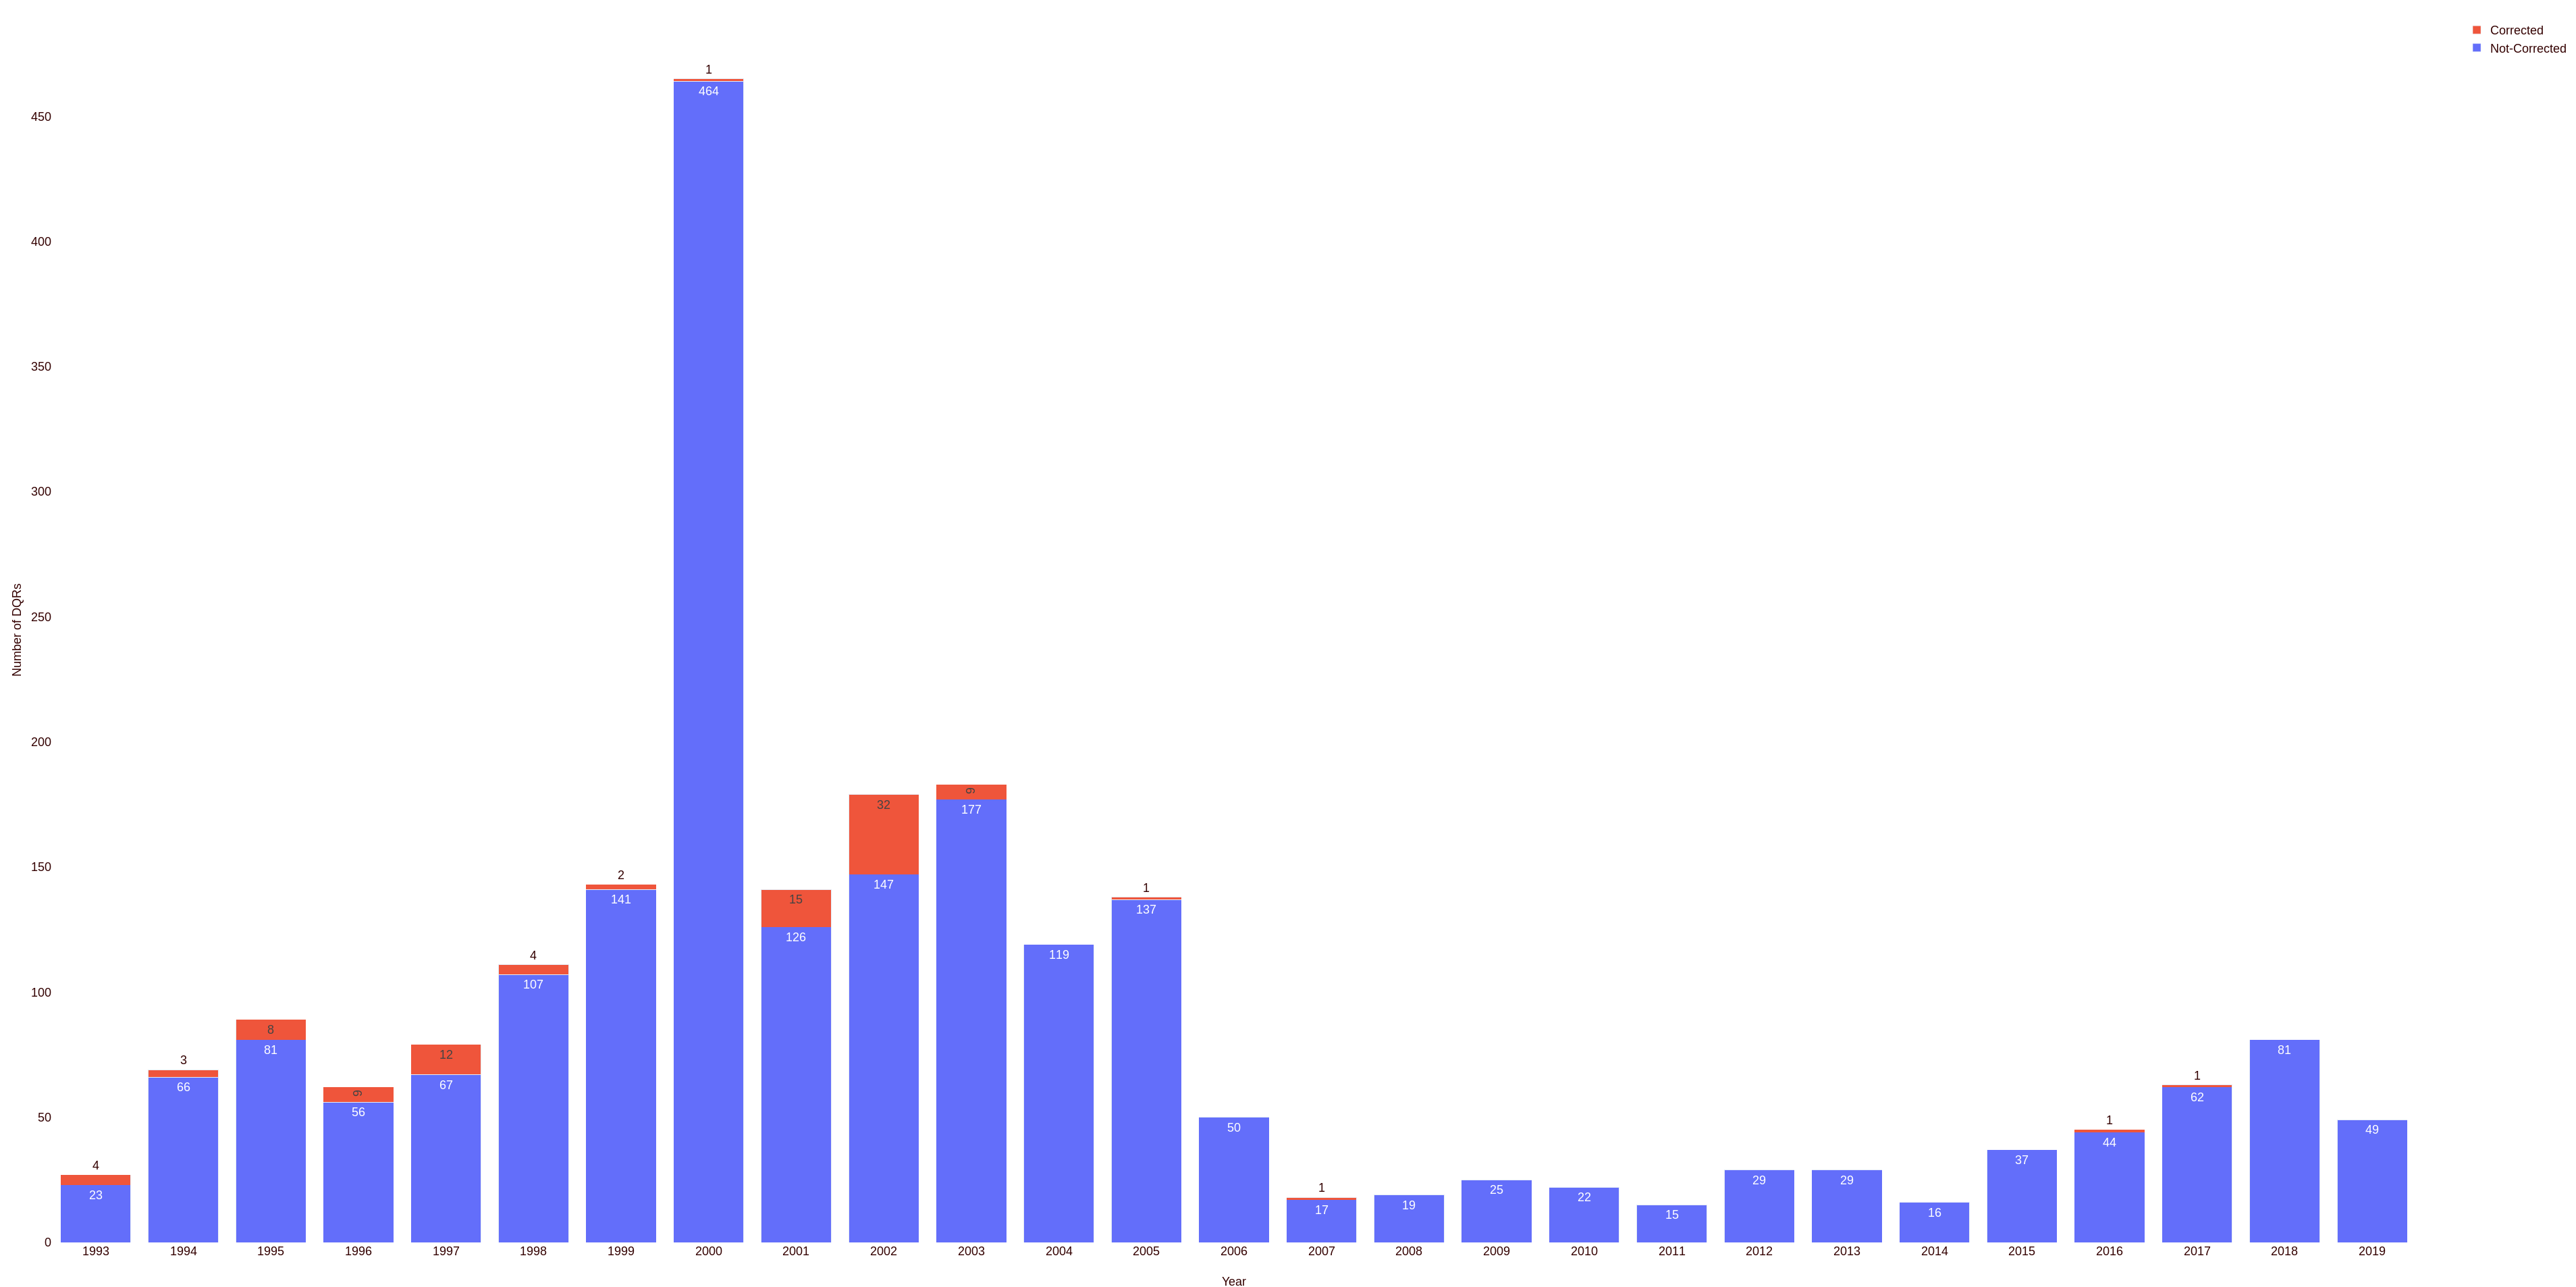
\includegraphics[width=\linewidth]{figures/30ebbr_dqr_reproc_by_year.png}
 }\\
 \subfloat[Surface Meteorology (MET) are another core instruments at ARM
 facilities that with frequent reported data quality issues, and
 many of them have been addressed in recent years as data quality
 improvement infrastructure has improved.]{
  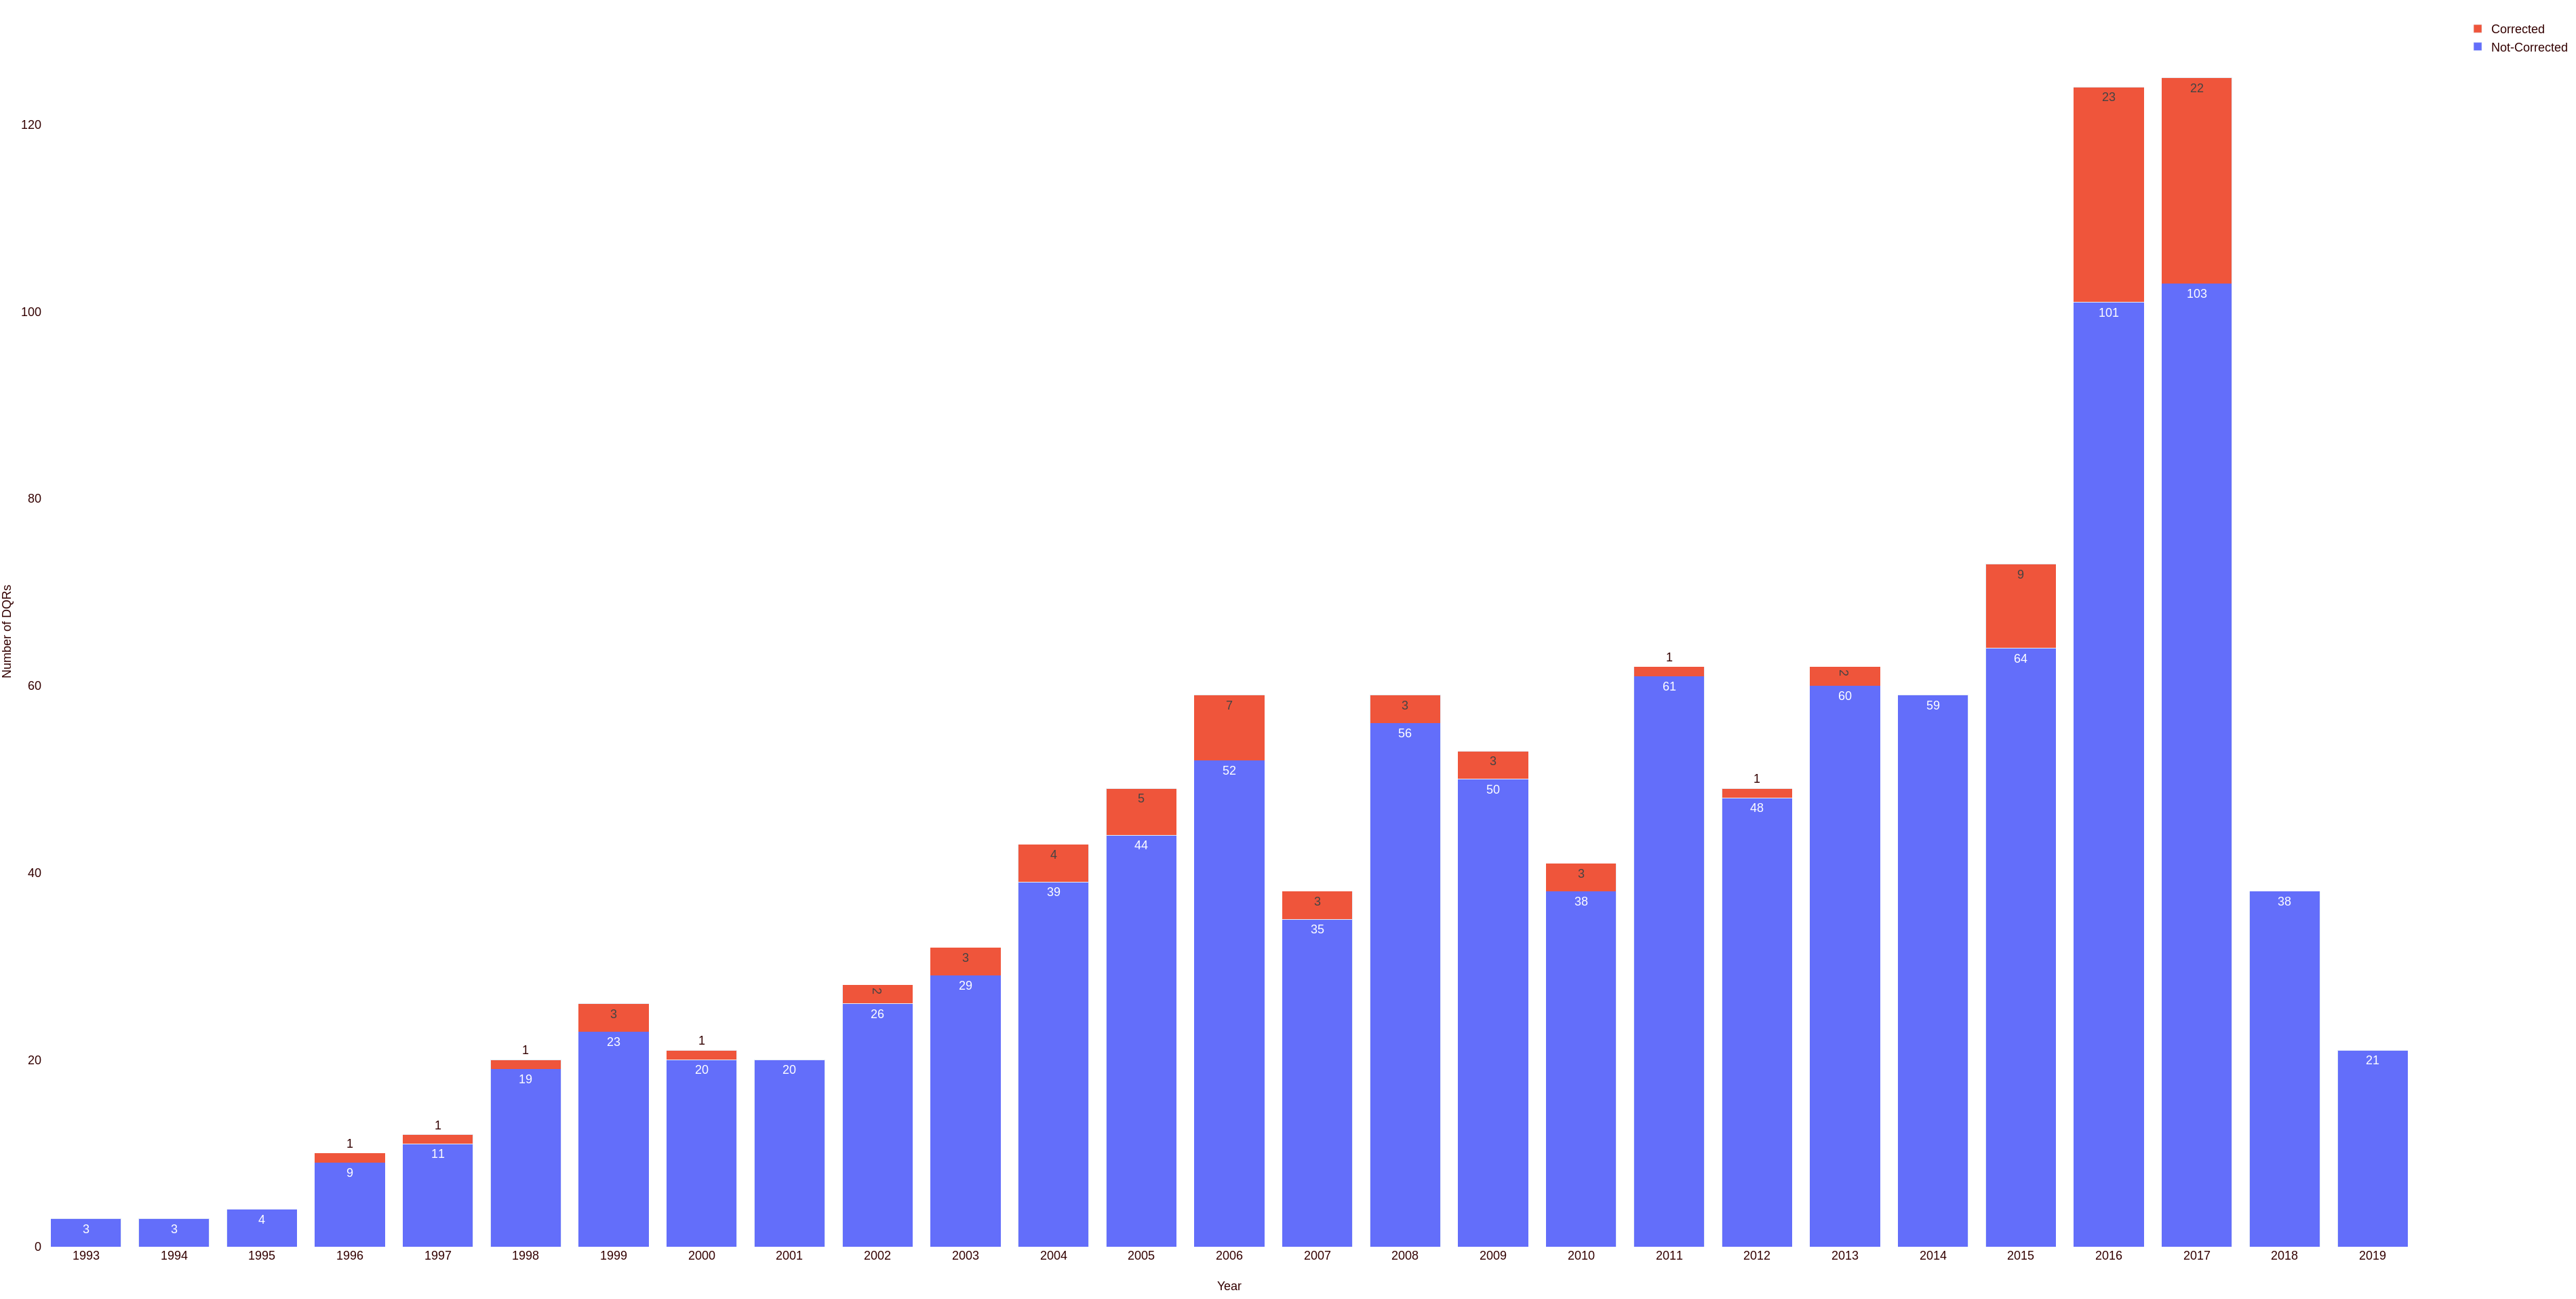
\includegraphics[width=\linewidth]{figures/met_dqr_reproc_by_year.png}
 }\\
 \subfloat[Radiation Measurements (RAD) instruments have had fairly
 small number of data quality issues, most of which have been addressed.]{
  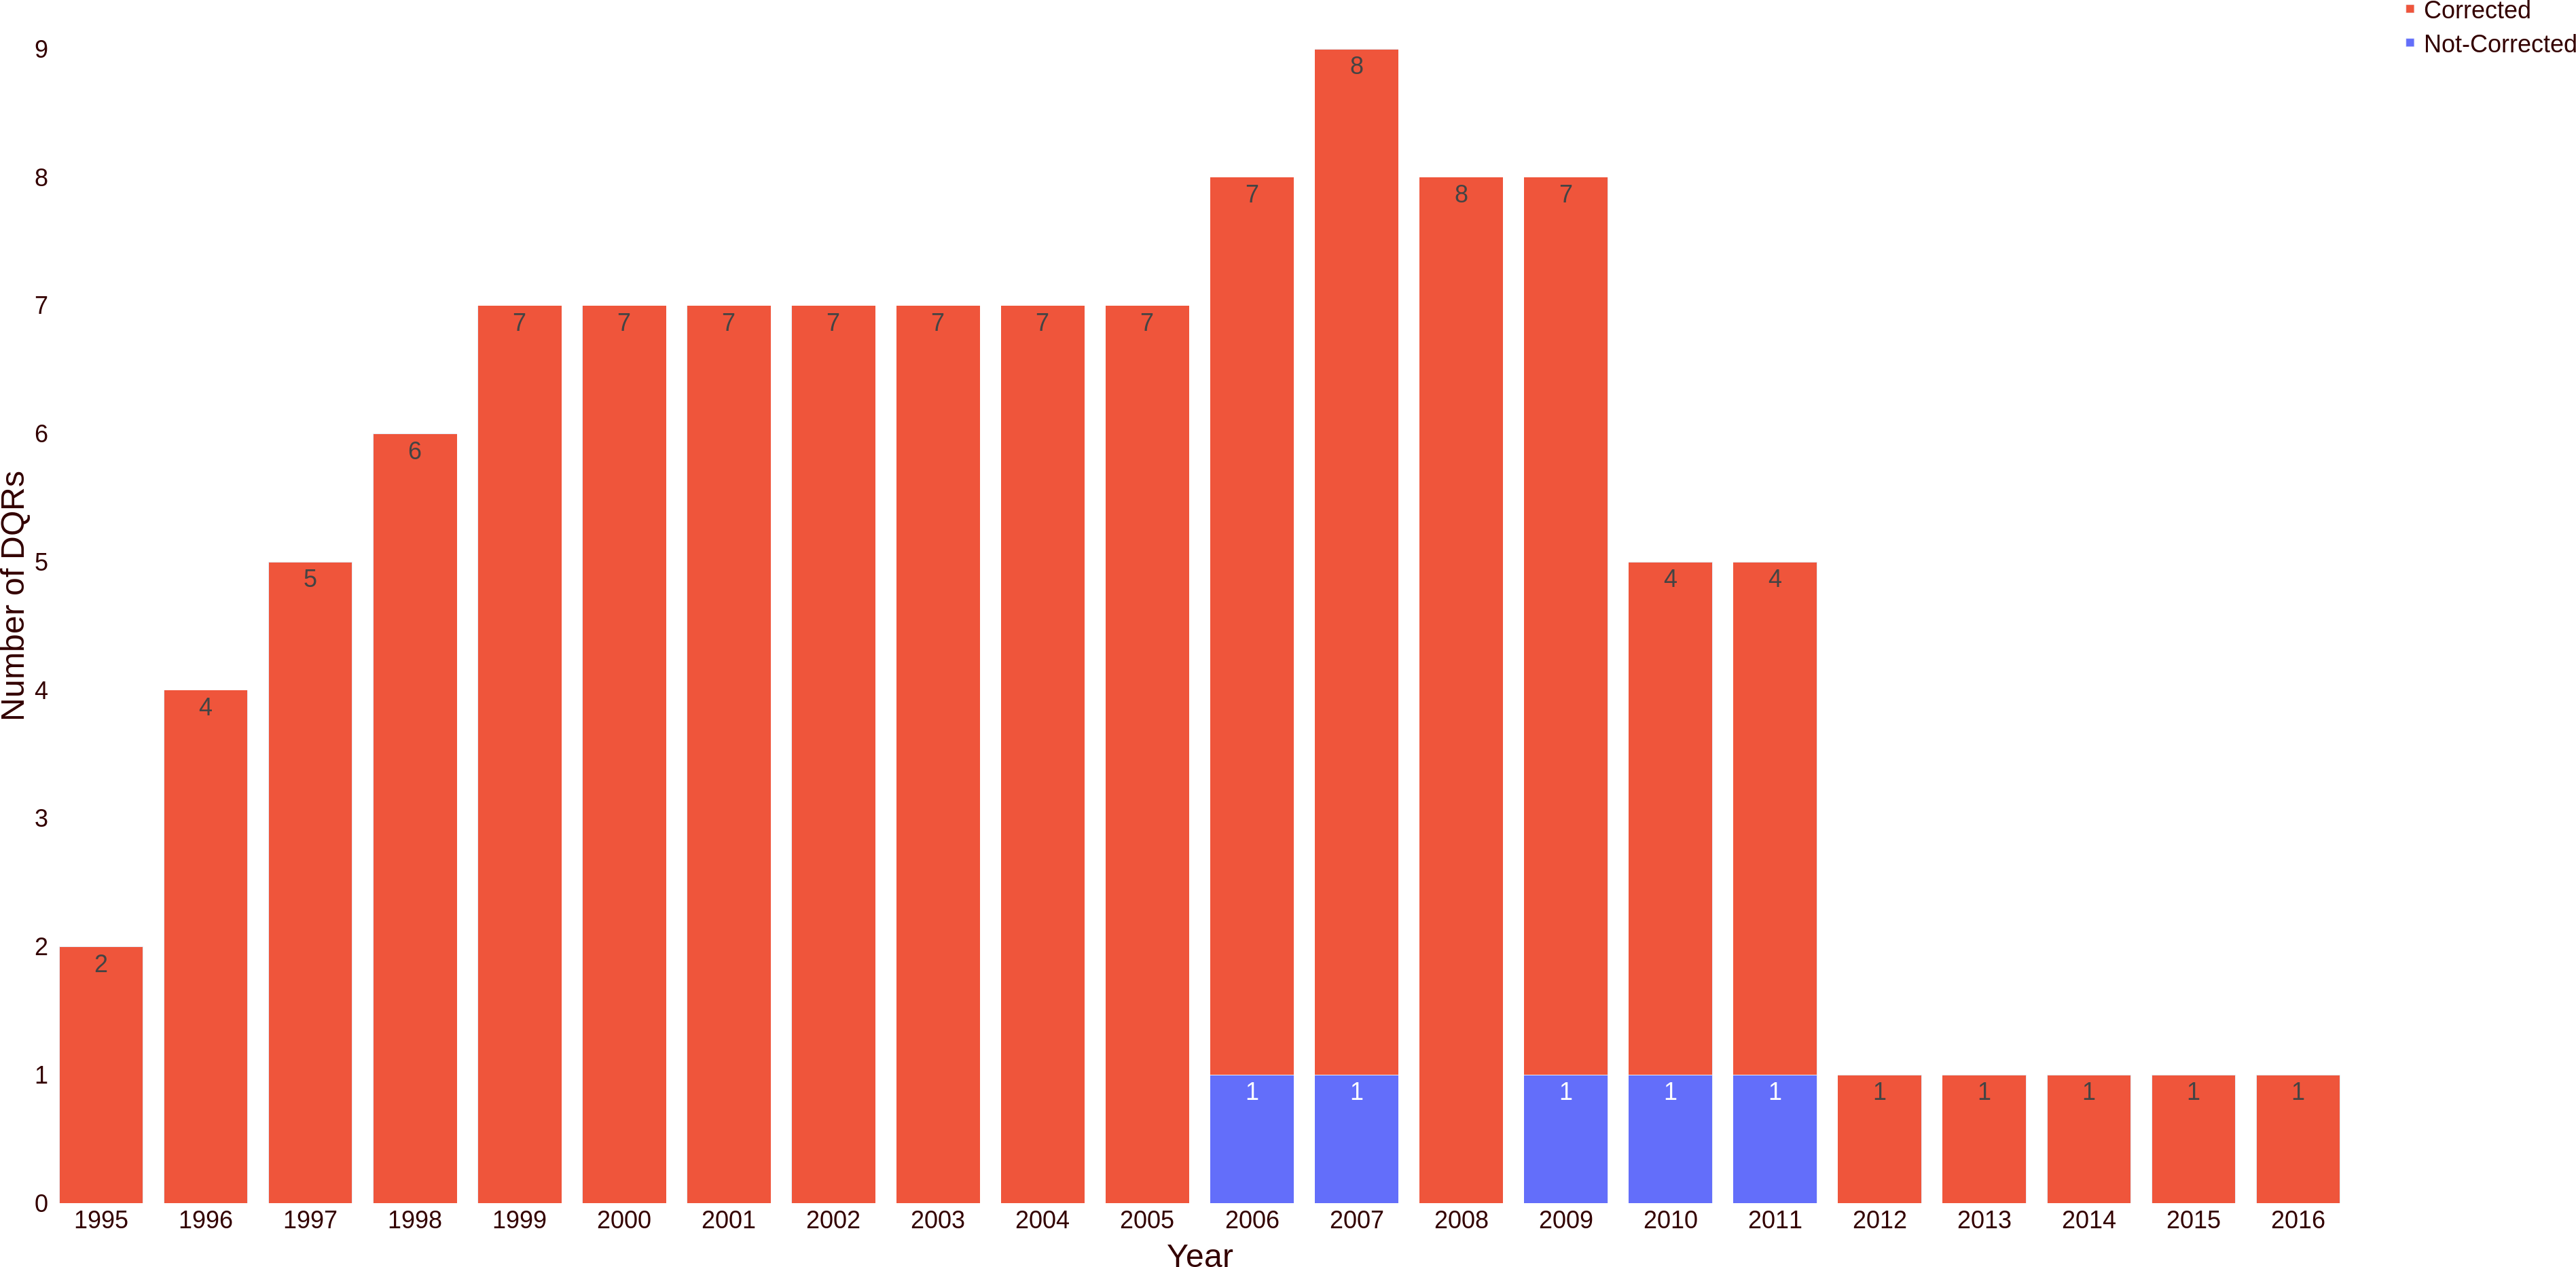
\includegraphics[width=\linewidth]{figures/radflux_dqr_reproc_by_year.png}
 }
 \caption{Only a small fraction of reported quality issues are corrected
 (shown in red) while majority remains uncorrected (shown in blue).
	 Fraction of corrected vs not-corrected are highly variable across
	 different instruments and are often determined by availability of
	 resolution for the issue, process complexity and data volume.}
 \label{fig:dqr_instrument_per_year}
\end{figure}
